\chapter{Исследовательский раздел}

Для проверки работоспособности разработанного ПО необходимо выполнить следующие действия:

\begin{itemize}
	\item На рисунке 4.1 демонстрируется сборка модуля, его загрузка, проверка
	сокрытия и выгрузка.
	\begin{figure}[H]
		\centering
		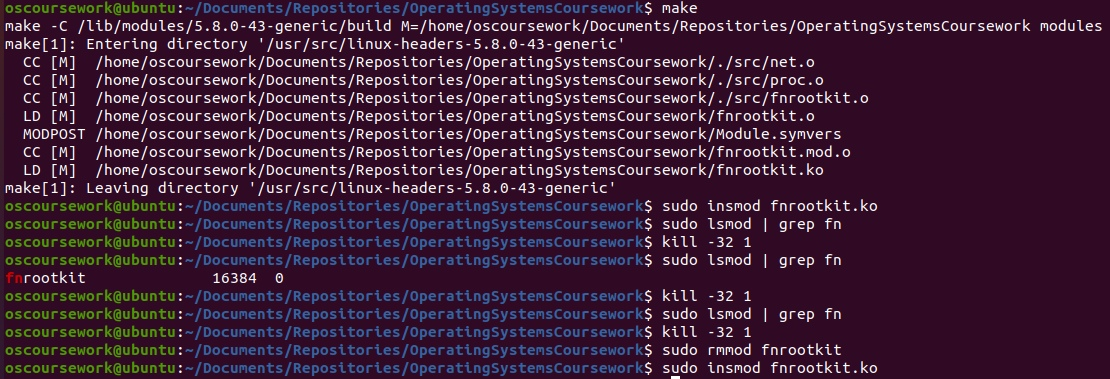
\includegraphics[scale=0.4]{inc/img/scr_01.jpg}
		\caption{Загрузка, сокрытие и выгрузка модуля}\label{img:module_hide}
	\end{figure}


	\item На рисунке 4.2 демонстрируется сокрытие процесса.
	\begin{figure}[H]
		\centering
		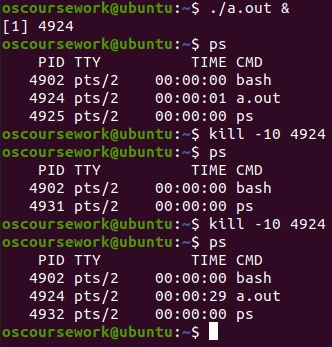
\includegraphics[scale=0.65]{inc/img/scr_02.jpg}
		\caption{Сокрытие процесса}\label{img:proc_hide}
	\end{figure}

	\item На рисунке 4.3 демонстрируется сокрытие сетевых сокетов.
	\begin{figure}[H]
		\centering
		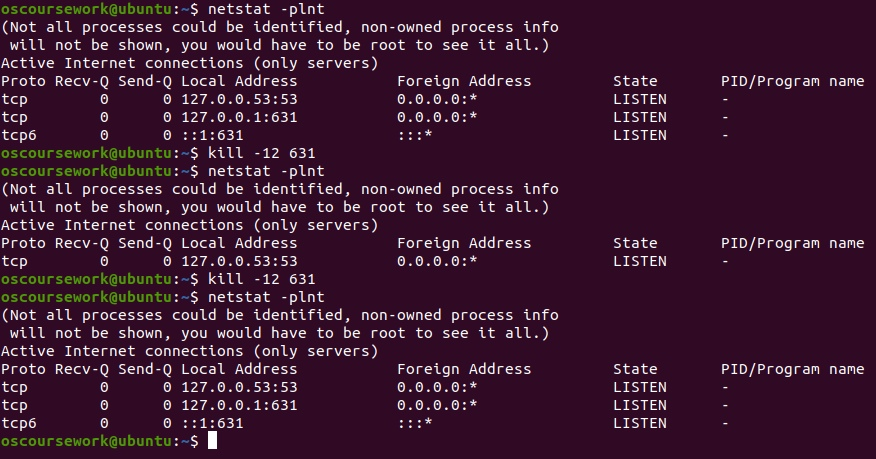
\includegraphics[scale=0.45]{inc/img/scr_03.jpg}
		\caption{Сокрытие сетевых сокетов}\label{img:net_hide}
	\end{figure}
\end{itemize}

\section*{Выводы}

Были показаны результаты работы ПО. В ходе тестирования не было
выявлено ошибок.